\newcommand*{\by}[0]{{\cellcolor{Orange!30}}}
\newcommand*{\py}[0]{{\cellcolor{NavyBlue!30}}}
\newcommand*{\wrng}[1]{{\cellcolor{Red!70}}\textcolor{white}{#1 X}}

\let\bnot\xoverline

\begin{enumerate}[label={[OH\arabic*]},start=15,leftmargin=0cm]
    \item 
        \begin{enumerate}[label={(\alph*)}]
            \item Die letzte zwei Ziffern meiner Matrikelnummer entspricht $43$, somit ist $X = 43$ und $Y = 43 + 57 = 100$. $$(100)_{10} = (0110 \, 0100)_2$$Wir konstruieren nun das entsprechende $12$-Bit Codewort:
                \begin{center}
                    \ttfamily\small
                    \begin{tabular}{l *{12}{c} l}
\toprule
              &  01 &  02 &  03 &  04 &  05 &  06 &  07 &  08 &  09 &  10 &  11 &  12 & Prüf\\
\midrule
Codewort:     &\py ?&\py ?&\by 0&\py ?&\by 1&\by 1&\by 0&\py ?&\by 0&\by 1&\by 0&\by 0& \\
\midrule
Parity Bit 1: &\py ?&     &\by 0&     &\by 1&     &\by 0&     &\by 0&     &\by 0&     & ? = 1\\
Parity Bit 2: &     &\py ?&\by 0&     &     &\by 1&\by 0&     &     &\by 1&\by 0&     & ? = 0\\
Parity Bit 4: &     &     &     &\py ?&\by 1&\by 1&\by 0&     &     &     &     &\by 0& ? = 0\\
Parity Bit 8: &     &     &     &     &     &     &     &\py ?&\by 0&\by 1&\by 0&\by 0& ? = 1\\
\midrule
Codewort:     &\py 1&\py 0&\by 0&\py 0&\by 1&\by 1&\by 0&\py 1&\by 0&\by 1&\by 0&\by 0& \\
\bottomrule
                    \end{tabular}
                \end{center}
                Das entsprechende $12$-Bit Codewort ist: $1000 \, 1101 \, 0100$.
            \item \blanko
                \vspace{-1.5\baselineskip}
                \begin{align*}
                    U &= 3 \\
                    V &= U + 1 = 3 + 1 = 4
                \end{align*}
                Wir kippen das Bit an der $4$-ten Stelle und das neue und ungültige Codewort ist:
            \begin{equation*}
                0101\,1111\,1011
            \end{equation*}
            Tabelle:
            \begin{center}
                    \ttfamily\small
                    \begin{tabular}{l *{12}{c} l}
\toprule
              &  01 &  02 &  03 &  04 &  05 &  06 &  07 &  08 &  09 &  10 &  11 &  12 & Prüf\\
\midrule
Codewort:     &\py 0&\py 1&\by 0&\py 1&\by 1&\by 1&\by 1&\py 1&\by 1&\by 0&\by 1&\by 1& \\
\midrule
Parity Bit 1: &\py 0&     &\by 0&     &\by 1&     &\by 1&     &\by 1&     &\by 1&     & :4\\
Parity Bit 2: &     &\py 1&\by 0&     &     &\by 1&\by 1&     &     &\by 0&\by 1&     & :4\\
Parity Bit 4: &     &     &     &\py 1&\by 1&\by 1&\by 1&     &     &     &     &\by 1& \wrng{:5} \\
Parity Bit 8: &     &     &     &     &     &     &     &\py 1&\by 1&\by 0&\by 1&\by 1& :4\\
\bottomrule
                    \end{tabular}
                \end{center}
            Die Prüfsumme des Paritätsbits 4 ist nun nicht mehr korrekt. Da Bit $4$ nur von Paritätsbit $4$ geprüft ist, ist nur das Paritätsbit $4$ falsch.
        \end{enumerate}
    \newpage
    \item 
        \begin{enumerate}[label={(\alph*)}]
            \item Wir davon aus, dass $Q$ und $\bnot{Q}$ in ihre Endzustand ohne jegliche Verzögerung geschaltet wird. Zudem gilt: 
                \begin{itemize}
                    \item Ist $D = 1$, dann $Q = 1, \bnot{Q} = 0$
                    \item Ist $D = 0$, dann $Q = 0, \bnot{Q} = 1$
                \end{itemize}
                egal, was der ursprungliche Zustand war. 

                Das Impulsdiagramm ist somit:
                \vspace{\baselineskip}
                \begin{center}
                    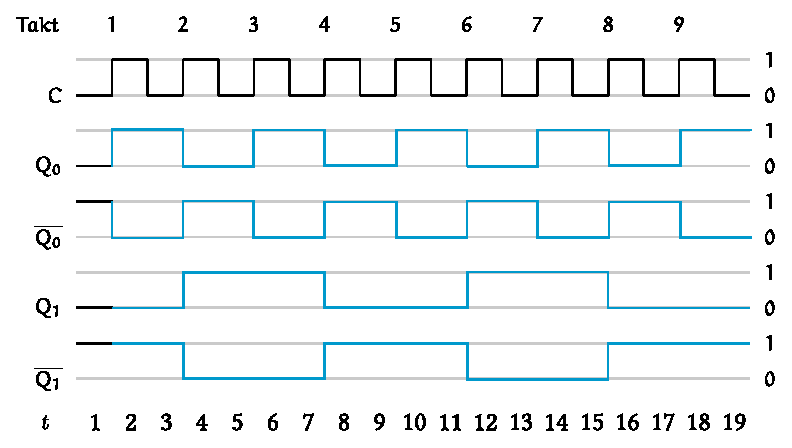
\includegraphics[width=0.85\textwidth]{flipflop.eps}
                \end{center}
                \vspace{\baselineskip}

            \item Seien:
                \begin{align*}
                    N_{C} &\coloneqq \text{Anzahl der Impulse im Taktsignal} \\
                    N_0 &\coloneqq \text{Anzahl der Impulse des Ausgangs } Q_0 \\
                    N_1 &\coloneqq \text{Anzahl der Impulse des Ausgangs } Q_1 
                \end{align*}
                Aus dem obigen Diagramm gilt:
                \begin{align*}
                    N_0 &= \floor*{\frac{N_{C}}{2}}  \\
                    N_1 &= \floor*{\frac{N_0}{2}}  = \floor*{\frac{N_{C}}{4}}
                \end{align*}
                Mit jedem weiteren D-Flipflop in dieser Reihenfolge wird die Anzahl der Impulse halbiert. 

                \newpage
                Mit diesem Aufbau kann man einen Zähler realisieren. Für jeden Zeitpunkt $t$, betrachten wir die Ausgänge $Q_1$, $Q_0$ und $C$:
                \vspace{\baselineskip}
                \begin{center}
                    \ttfamily
                    \begin{tabular}{l lll r}
                        \toprule
                        $t$ & $Q_1$ & $Q_0$ & $C$ & \textnormal{Zähler} \\
                        \midrule
                        01 & 0 & 0 & 0 & 0 \\
                        02 & 0 & 0 & 1 & 1 \\
                        03 & 0 & 1 & 0 & 2 \\
                        04 & 0 & 1 & 1 & 3 \\
                        05 & 1 & 0 & 0 & 4 \\
                        06 & 1 & 0 & 1 & 5 \\
                        07 & 1 & 1 & 0 & 6 \\
                        08 & 1 & 1 & 1 & 7 \\
                        \hdashline
                        09 & 0 & 0 & 0 & 0 \\
                        10 & 0 & 0 & 1 & 1 \\
                        11 & 0 & 1 & 0 & 2 \\
                        12 & 0 & 1 & 1 & 3 \\
                        13 & 1 & 0 & 0 & 4 \\
                        14 & 1 & 0 & 1 & 5 \\
                        15 & 1 & 1 & 0 & 6 \\
                        16 & 1 & 1 & 1 & 7 \\
                        \hdashline
                        17 & 0 & 0 & 0 & 0 \\
                        18 & 0 & 0 & 1 & 1 \\
                        19 & 0 & 1 & 0 & 2 \\
                        \bottomrule
                    \end{tabular}
                \end{center}
            \vspace{\baselineskip}
            Wenn man $(Q_1, Q_0, C)$ als Binärdarstellung einer Zahl betrachtet, dann haben wir einen Zähler, die von $0$ bis $7$ abzählt. Nach $7$ ist der Zähler auf $0$ zurückgesetzt und der Zyklus wiederholt sich. 

            Braucht man das Taktsignal (jede zweite Zeile), dann haben wir nur einen Zähler $(Q_1, Q_0)$, die von $0$ bis $3$ abzählt. 

            % https://www.eecs.tufts.edu/~dsculley/tutorial/flopsandcounters/flops5.html
        \end{enumerate}
\end{enumerate}